% !TEX program = xelatex
\documentclass[12pt,a4paper]{article}

% =================== PACKAGES ===================
\usepackage[T1]{fontenc}
\usepackage{geometry}
\usepackage{graphicx}
\usepackage{hyperref}
\usepackage{enumitem}
\usepackage{titlesec}
\usepackage{fancyhdr}
\usepackage{booktabs}
\usepackage{array}
\usepackage{tabularx}
\usepackage{longtable}
\usepackage{setspace}
\usepackage[final,nopatch=footnote]{microtype}
\usepackage{newtxtext}
\usepackage{parskip}
\usepackage[nottoc]{tocbibind}
\usepackage{tikz}
\usetikzlibrary{arrows.meta, positioning, shapes.geometric, backgrounds, calc, fit, matrix}
\usepackage{caption}
\captionsetup{font=small, labelfont=bf, margin=0.5cm}
\usepackage{float}
\usepackage{xcolor}
\usepackage{pdflscape}
\usepackage{ragged2e}
% \usepackage{makecell}  % removed --- not needed
% \usepackage{multirow}  % removed --- not needed
\graphicspath{{img/}}

% =================== PAGE LAYOUT ===================
\geometry{
  top=1in,
  bottom=1in,
  left=1.05in,
  right=1.05in,
  headheight=14pt,
  headsep=18pt
}
\setstretch{1.12}
\setlength{\emergencystretch}{3em}

% =================== COLOURS ===================
\definecolor{lkblue}{HTML}{1F5B8F}
\definecolor{lkcyan}{HTML}{E9F4FB}
\definecolor{lkgreen}{HTML}{2E7D32}
\definecolor{lkorange}{HTML}{C46A1A}
\definecolor{lkpurple}{HTML}{6A4C93}
\definecolor{lkgray}{HTML}{F4F6F8}
\definecolor{darkgray}{HTML}{333333}

% =================== HEADER / FOOTER ===================
\pagestyle{fancy}
\fancyhf{}
\fancyhead[L]{\small IK2015 Enterprise Architecture}
\fancyhead[R]{\small Seminar 6: ArchiMate Layered Architecture \& Schema Refinement}
\fancyfoot[C]{\thepage}
\renewcommand{\headrulewidth}{0.4pt}

% =================== SECTION FORMATTING ===================
\titleformat{\section}[hang]{\Large\bfseries\color{darkgray}}{\thesection}{1em}{}
\titleformat{\subsection}[hang]{\large\bfseries\color{darkgray}}{\thesubsection}{1em}{}
\titleformat{\subsubsection}[hang]{\normalsize\bfseries\color{darkgray}}{\thesubsubsection}{1em}{}
\titlespacing*{\section}{0pt}{12pt}{6pt}
\titlespacing*{\subsection}{0pt}{10pt}{4pt}
\titlespacing*{\subsubsection}{0pt}{8pt}{2pt}

% =================== HYPERLINK SETUP ===================
\hypersetup{
  colorlinks=true,
  linkcolor=black,
  citecolor=black,
  urlcolor=lkblue,
  pageanchor=false
}

% =================== TABLE HELPERS ===================
\newcolumntype{Y}{>{\RaggedRight\arraybackslash}X}
\newcolumntype{P}[1]{>{\RaggedRight\arraybackslash}p{#1}}
\renewcommand{\arraystretch}{1.22}
\newcommand{\pk}[1]{\underline{#1}}
\newcommand{\fk}{\textsuperscript{FK}}
\newcommand{\pkfk}{\textsuperscript{PK, FK}}
\newcommand{\nullable}{\textsuperscript{nullable}}

% =================== TITLE AREA ===================
\title{}
\author{}
\date{}

\begin{document}

% ---- Custom Title Page ----
\thispagestyle{empty}
\vspace*{1.8cm}

\begin{center}
  {\normalsize Jiangxi University of Finance and Economics} \\[2.1cm]

  {\LARGE\bfseries ArchiMate Layered Architecture and} \\[0.15cm]
  {\LARGE\bfseries Relational Schema Refinement} \\[0.15cm]
  {\LARGE\bfseries Report} \\[1.0cm]

  {\Large Luckin Coffee Inc.} \\[0.25cm]
  {\normalsize\itshape A Technology-Driven New Retail Coffee Enterprise} \\[2.0cm]

  {\normalsize IK2015: Enterprise Architecture and Database Programming} \\[0.2cm]
  {\normalsize Seminar 6} \\[2.2cm]

  {\normalsize\textbf{Group 4}} \\[0.45cm]
  {\normalsize
    Zhe-Kai Yang~(Krust),\quad
    Shi-Hang Chen~(Sean),\quad
    Wei-Yu Cai~(Nosta), \\[0.2cm]
    Huan-Wen Chen~(Evan),\quad
    Yuan-Yong Liao~(Foreve)
  } \\[1.8cm]

  {\normalsize \today}
\end{center}

\newpage
\hypersetup{pageanchor=true}
\setcounter{page}{1}
\pagenumbering{arabic}
\pagestyle{fancy}

% =================== BASIC INFORMATION ===================
\section{Report Basic Information}

\begin{table}[H]
\centering
\caption{Basic information of the Seminar 6 report.}
\begin{tabularx}{\textwidth}{P{4.25cm}Y}
\toprule
\textbf{Item} & \textbf{Information} \\
\midrule
Selected enterprise / business & Luckin Coffee Inc.; mobile-first coffee retail, pickup, delivery, partnership-store operation, and packaged coffee business. \\
Course and seminar & IK2015 Enterprise Architecture and Database Programming; Seminar 6. \\
Group number & Group 4. \\
Group members & \parbox[t]{\hsize}{\raggedright Zhe-Kai Yang~(Krust), Shi-Hang Chen~(Sean), Wei-Yu Cai~(Nosta),\\ Huan-Wen Chen~(Evan), Yuan-Yong Liao~(Foreve).} \\
Main deliverable & ArchiMate layered architecture diagrams (Business, Application, Technology) for Luckin Coffee and refined relational schema with normalization documentation. \\
Connects to & \begin{itemize}[leftmargin=*, nosep, label=-]
    \item Seminar 4 --- Conceptual ER model (source for relational mapping).
    \item Seminar 5 --- Zachman Row 1 Scope and initial relational data model.
\end{itemize} \\
\bottomrule
\end{tabularx}
\end{table}

This report follows the Seminar 6 instruction sheet. It first presents three Archi\-Mate layered architecture views — Business Layer Model (BLM), Application Layer Model (ALM), and Technology Layer Model (TLM) — that describe the Luckin Coffee enterprise architecture from stakeholder-facing business processes down to a proposed technology deployment view. It then refines the relational data model from Seminar 5, documenting normalization to Third Normal Form (3NF), a data dictionary, sample data, and the final relational schema.

% =================== PART I: ARCHITECTURE MODELS ===================
\section{ArchiMate Layered Architecture Models}

Enterprise architecture describes an organization through multiple layers of abstraction. Following the ArchiMate modelling standard, this section presents the Luckin Coffee architecture across three layers: the Business Layer (actors, services, processes), the Application Layer (application services, components, data objects), and the Technology Layer (devices, networks, platform software, and infrastructure artifacts). The Business and Application layers are modelled from the observable Luckin business model and digital service pattern. The Technology Layer is a proposed / assumed deployment architecture for Luckin Coffee based on that digital retail business model; it should not be read as a confirmed disclosure of Luckin Coffee's internal production infrastructure.

\subsection{Business Layer Model (BLM)}

The Business Layer describes the enterprise from the perspective of business actors, roles, services, processes, and objects. It answers the question: \textit{what does the business do, who is involved, and how is value delivered?}

\begin{figure}[H]
\centering
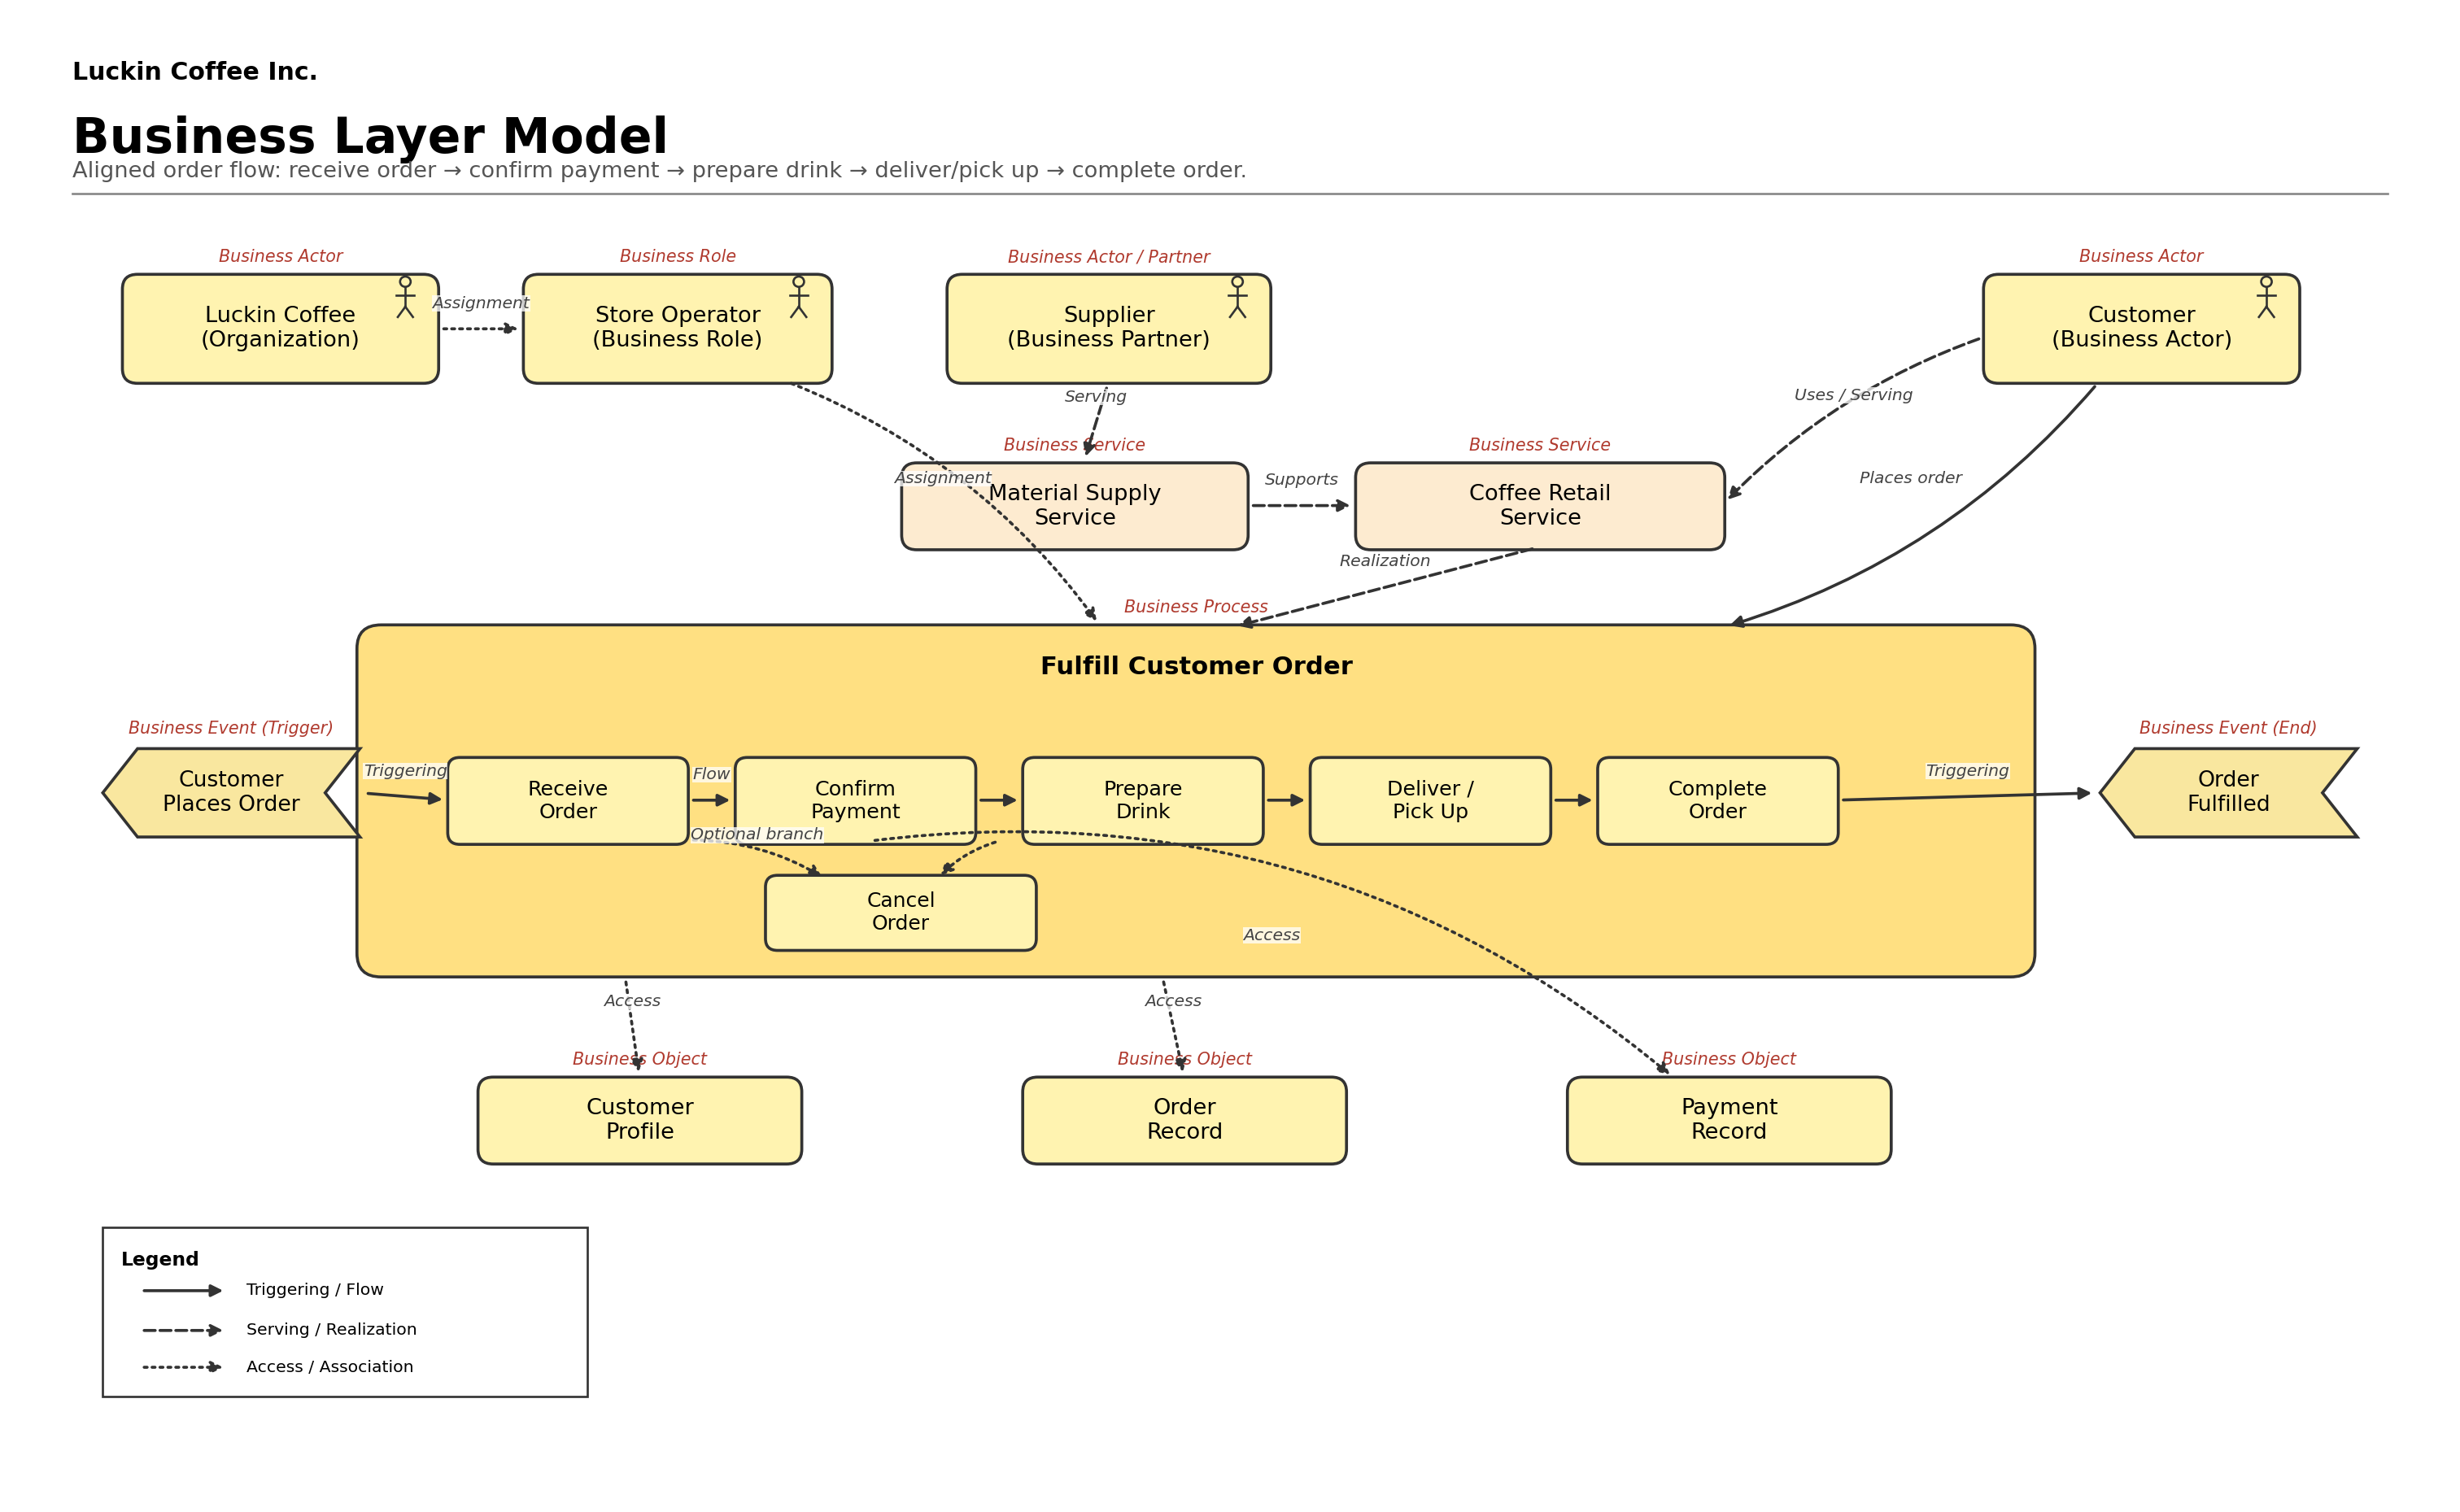
\includegraphics[width=\linewidth,keepaspectratio]{BLM.png}
\caption{Business Layer Model for Luckin Coffee --- showing business actors, roles, the core coffee retail service, and the Fulfill Customer Order business process.}
\label{fig:blm}
\end{figure}

\subsubsection{Business Actors and Roles}

\begin{table}[H]
\centering
\caption{Business actors and roles in the BLM.}
\small
\begin{tabularx}{\textwidth}{P{3.5cm}P{2.8cm}Y}
\toprule
\textbf{Element} & \textbf{ArchiMate Type} & \textbf{Description} \\
\midrule
Luckin Coffee & Organization & The enterprise itself --- the legal entity that owns the brand, platform, and operating model. \\
Store Operator & Business Role & The operational role responsible for managing store resources, staff scheduling, and physical fulfilment. \\
Supplier & Business Actor / Partner & External partner providing raw materials (coffee beans, milk, syrup, packaging), equipment, and recipe input. \\
Customer & Business Actor & The end consumer who places orders, receives beverages, and provides feedback. \\
\bottomrule
\end{tabularx}
\end{table}

\subsubsection{Business Service}

The model identifies one core business service: \textbf{Coffee Retail Service}. This service encapsulates the value Luckin delivers --- freshly brewed coffee and tea beverages, fulfilled through pickup or delivery channels, at affordable prices. The Supplier is assigned to support this service, reflecting the integral role of raw-material sourcing in product quality.

\subsubsection{Business Process: Fulfill Customer Order}

The central business process is \textbf{Fulfill Customer Order}, which decomposes into five sub-processes. In Luckin's usual digital ordering scenario, payment confirmation happens before store preparation and pickup or delivery:

\begin{enumerate}[leftmargin=1.3em, nosep]
  \item \textbf{Receive Order} --- The customer initiates an order via the mobile app, WeChat mini-program, or other digital channel. The order is captured, validated, and routed to the appropriate store.
  \item \textbf{Confirm Payment} --- The system confirms that the digital payment has succeeded or that an approved payment method has been authorized before fulfilment starts.
  \item \textbf{Prepare Drink} --- Store staff follow standardized recipes to prepare the ordered beverage. Equipment sensors (IoT) may monitor preparation parameters.
  \item \textbf{Deliver or Pick Up} --- The completed order is either handed to the customer for in-store pickup or handed to a delivery rider for last-mile delivery.
  \item \textbf{Complete Order} --- The fulfilment result is recorded after successful pickup or delivery, and the order status is closed.
\end{enumerate}

The process is triggered by the business event \textbf{Customer Places Order} and terminates with the end event \textbf{Order Fulfilled}. The business object \textbf{Customer Profile} is accessed by the Customer actor, linking identity and preference data to the service.

\subsubsection{Process Flow Diagram}

\begin{center}
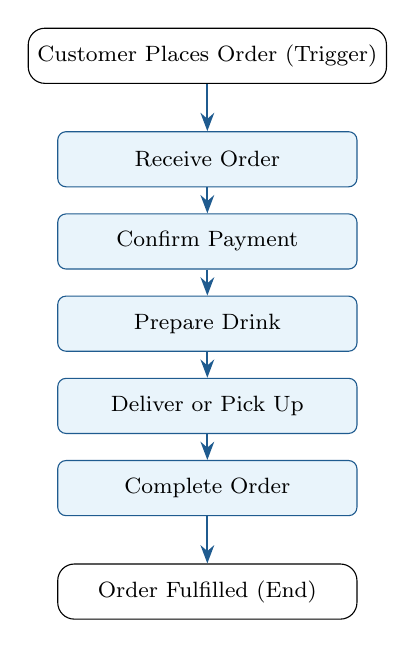
\begin{tikzpicture}[
    node distance=1.4cm,
    box/.style={rectangle, draw=lkblue, fill=lkcyan, rounded corners=3pt, minimum width=3.8cm, minimum height=0.7cm, font=\footnotesize},
    event/.style={rectangle, draw=black, fill=white, rounded corners=6pt, minimum width=3.8cm, minimum height=0.7cm, font=\footnotesize},
    arrow/.style={->, >=Stealth, thick, draw=lkblue}
  ]
  \node[event] (trigger) {Customer Places Order (Trigger)};
  \node[box, below=0.6cm of trigger] (receive) {Receive Order};
  \node[box, below=0.33cm of receive] (payment) {Confirm Payment};
  \node[box, below=0.33cm of payment] (prepare) {Prepare Drink};
  \node[box, below=0.33cm of prepare] (deliver) {Deliver or Pick Up};
  \node[box, below=0.33cm of deliver] (complete) {Complete Order};
  \node[event, below=0.6cm of complete] (end) {Order Fulfilled (End)};

  \draw[arrow] (trigger) -- (receive);
  \draw[arrow] (receive) -- (payment);
  \draw[arrow] (payment) -- (prepare);
  \draw[arrow] (prepare) -- (deliver);
  \draw[arrow] (deliver) -- (complete);
  \draw[arrow] (complete) -- (end);
\end{tikzpicture}
\end{center}

\subsection{Application Layer Model (ALM)}

The Application Layer describes the software services, application components, and data objects that realize the business processes. It answers the question: \textit{what applications support the business, and how do they manage data?}

\begin{figure}[H]
\centering
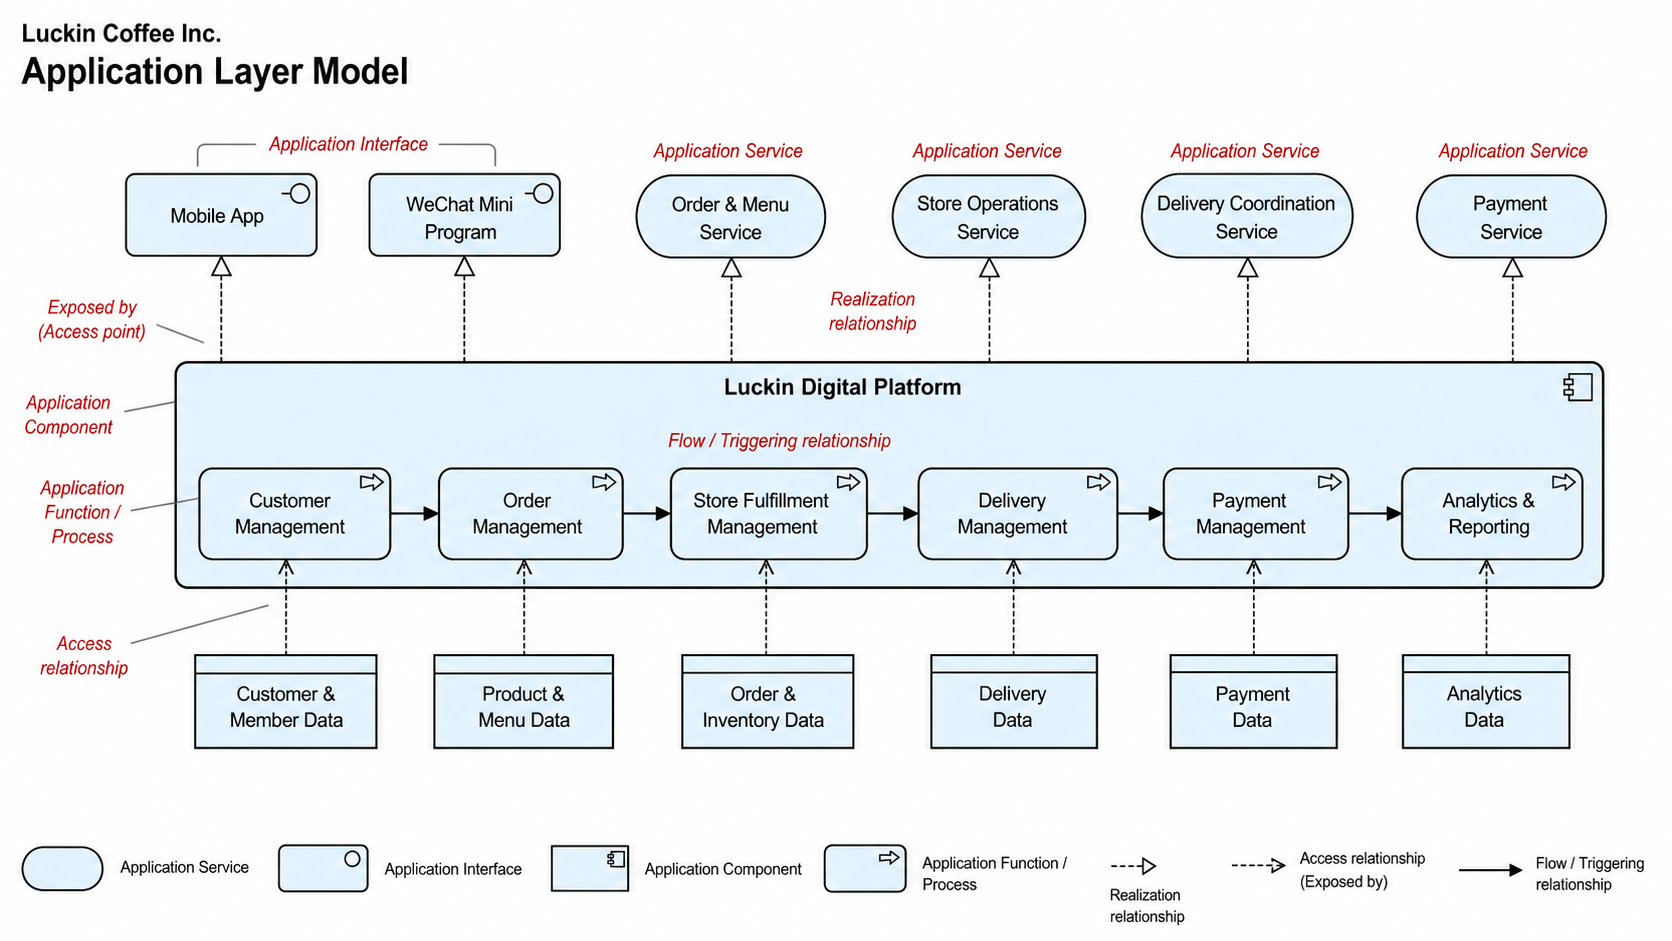
\includegraphics[width=\linewidth,keepaspectratio]{ALM.png}
\caption{Application Layer Model for Luckin Coffee --- showing customer-facing application interfaces, application services, a logical Luckin Digital Platform decomposition, and managed data objects.}
\label{fig:alm}
\end{figure}

\subsubsection{Application Interfaces}

In ArchiMate, an \textbf{Application Interface} is the mechanism through which a user or external system accesses an Application Service. The ALM identifies two primary customer-facing application interfaces:

\begin{table}[H]
\centering
\caption{Application interfaces in the ALM.}
\small
\begin{tabularx}{\textwidth}{P{3.2cm}P{2.6cm}Y}
\toprule
\textbf{Interface} & \textbf{Type} & \textbf{Description} \\
\midrule
Mobile App & iOS / Android Application & Primary customer-facing interface for browsing the menu, placing orders, managing membership, receiving promotions, and tracking order status. \\
WeChat Mini Program & Mini Program & Lightweight alternative ordering interface embedded in the WeChat ecosystem, reducing the friction of app installation. \\
\bottomrule
\end{tabularx}
\end{table}


\subsubsection{Application Services}

The ALM exposes four backend application services, each realizing a distinct business capability:

\begin{table}[H]
\centering
\caption{Application services in the ALM.}
\small
\begin{tabularx}{\textwidth}{P{3.2cm}P{2.6cm}Y}
\toprule
\textbf{Service} & \textbf{Type} & \textbf{Description} \\
\midrule
Order \& Menu Service & Application Service & Manages the product catalogue (menu), order creation, order routing to stores, and order status lifecycle. \\
Store Operations Service & Application Service & Supports store-level functions: queue management, preparation workflow, inventory checks, and staff task assignment. \\
Delivery Coordination Service & Application Service & Coordinates last-mile delivery: rider assignment, route optimization, estimated delivery time, and delivery status tracking. \\
Payment Service & Application Service & Processes digital payments across multiple methods (WeChat Pay, Alipay, bank card), records transactions, and handles refunds. \\
\bottomrule
\end{tabularx}
\end{table}

\subsubsection{Application Components: Luckin Digital Platform}

For modelling purposes, the platform is decomposed into six logical application components, each encapsulating a cohesive set of business logic:

\begin{table}[H]
\centering
\caption{Application components within the Luckin Digital Platform.}
\small
\begin{tabularx}{\textwidth}{P{3.6cm}Y}
\toprule
\textbf{Component} & \textbf{Responsibilities} \\
\midrule
Customer Management & Customer registration, profile management, membership tiering, points accounting, coupon wallet, and preference tracking. \\
Order Management & Order creation and validation, order assignment to stores, status tracking, queue management, and order lifecycle from placement to completion. \\
Store Fulfillment Management & Store-level preparation workflow, recipe display, equipment integration, task queue, and completion confirmation. \\
Delivery Management & Rider assignment, delivery route optimization, real-time tracking, estimated time of arrival, and delivery completion recording. \\
Payment Management & Payment processing, transaction logging, refund handling, settlement with payment providers, and payment risk-control support. \\
Analytics \& Reporting & Business intelligence dashboards, sales reports, customer behaviour analysis, campaign effectiveness measurement, and operational KPI computation. \\
\bottomrule
\end{tabularx}
\end{table}

The flow relationships connect application interfaces and services to the components they invoke: the Mobile App and WeChat Mini Program interfaces both serve as access points to the Order \& Menu Service, which flows to Order Management; Store Operations Service flows to Store Fulfillment Management; Delivery Coordination Service flows to Delivery Management; and Payment Service flows to Payment Management.

\subsubsection{Data Objects}

Each application component manages one or more data objects. These data objects correspond directly to the entities that will be modelled in the relational schema:

\begin{table}[H]
\centering
\caption{Data objects and their mapping to database tables.}
\small
\begin{tabularx}{\textwidth}{P{3.8cm}P{3.8cm}Y}
\toprule
\textbf{Data Object} & \textbf{Maps to Table(s)} & \textbf{Managed by} \\
\midrule
Customer \& Member Data & \texttt{Customers}, \texttt{MembershipAccounts} & Customer Management \\
Product \& Menu Data & \texttt{Products}, \texttt{RecipeStandards} & Order Management \\
Order \& Inventory Data & \texttt{DigitalOrders}, \texttt{OrderItems}, \texttt{StoreMaterials} & Order \& Store Management \\
Delivery Data & \texttt{FulfilmentTasks}, \texttt{DeliveryPartners} & Delivery Management \\
Payment Data & \texttt{Payments} (via Payment Service) & Payment Management \\
Analytics Data & Reporting views / OLAP store & Analytics \& Reporting \\
\bottomrule
\end{tabularx}
\end{table}

\subsection{Technology Layer Model (TLM)}

The Technology Layer describes a plausible physical and platform infrastructure --- devices, networks, platform hosting, system software, and technology artifacts --- on which the application components could run. Because Luckin Coffee does not publicly disclose every detail of its internal production infrastructure, this view is treated as a proposed / assumed deployment architecture rather than a verified inventory of actual systems.

\begin{figure}[H]
\centering
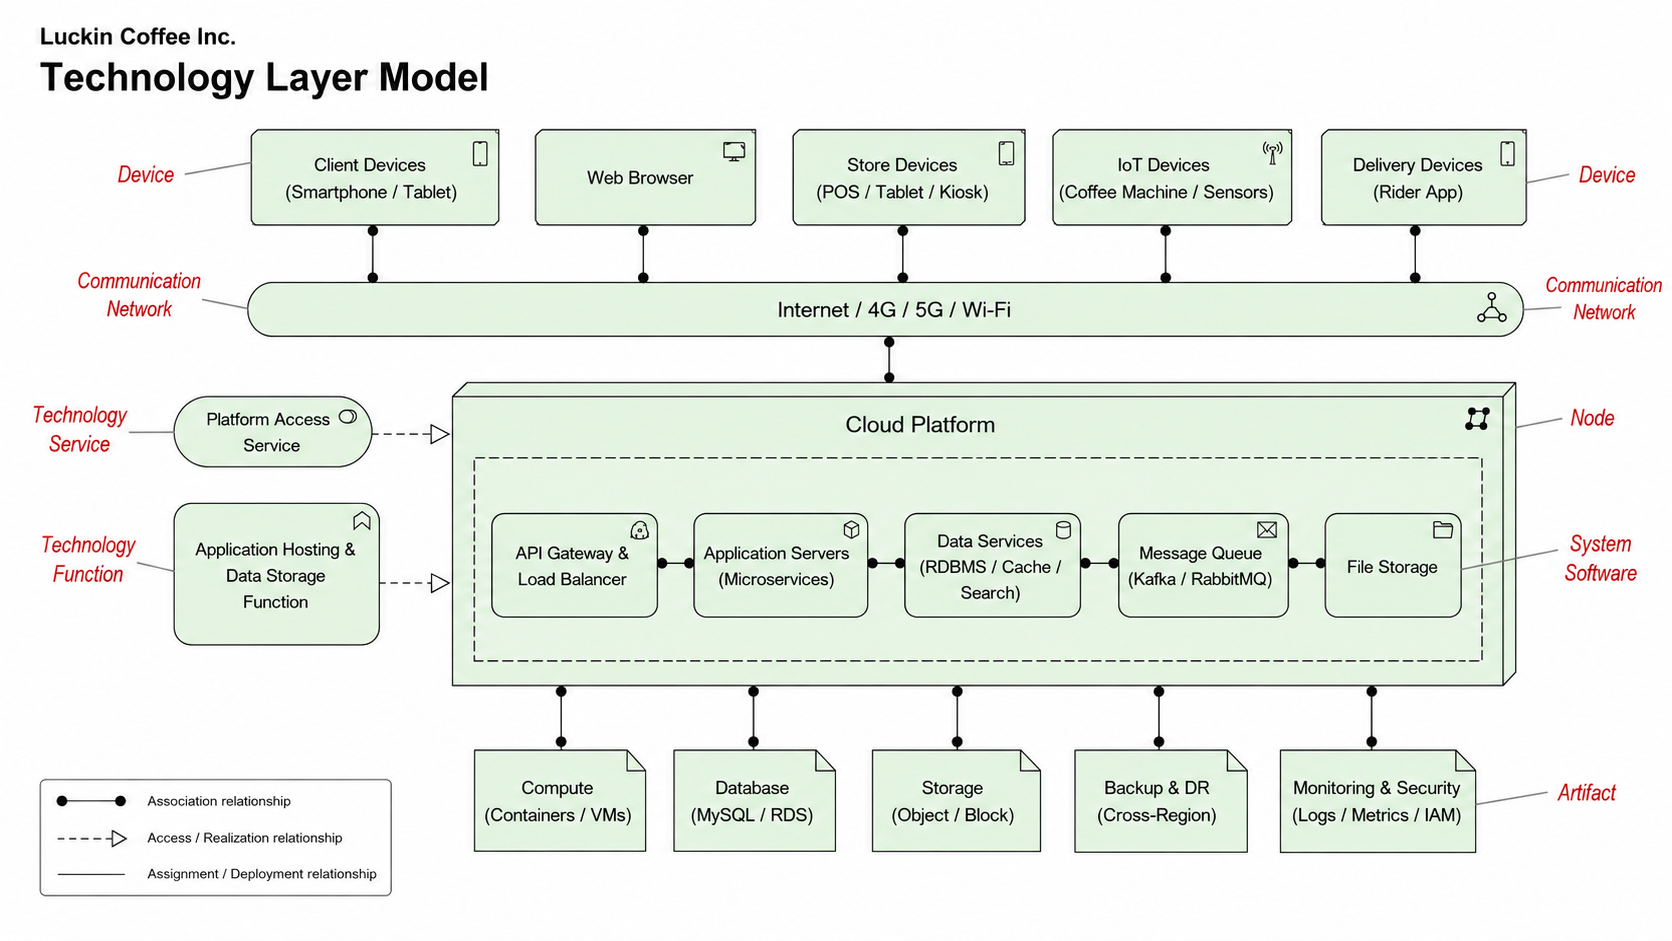
\includegraphics[width=\linewidth,keepaspectratio]{TLM.png}
\caption{Proposed Technology Layer Model for Luckin Coffee --- showing devices, communication networks, a cloud platform, system software, and technology artifacts in an assumed deployment architecture.}
\label{fig:tlm}
\end{figure}

\subsubsection{Device Layer}

Five categories of endpoint or infrastructure devices interact with the Luckin platform. Software entry points such as browsers and rider apps are represented as interfaces running on physical devices, rather than as devices themselves:

\begin{table}[H]
\centering
\caption{Device types in the TLM.}
\small
\begin{tabularx}{\textwidth}{P{3.2cm}P{3.0cm}Y}
\toprule
\textbf{Device} & \textbf{Type} & \textbf{Primary Users / Context} \\
\midrule
Client Device & Smartphone / Tablet & Customers for ordering; Store operators for fulfilment tasks. \\
Office PC / Laptop & Web Browser Interface & Internal staff (HQ planners, analysts, supply chain managers) access back-office functions through a browser running on a workstation. \\
Store Device & POS, Label Printer & Store staff for order receipt printing, label generation, and in-store point-of-sale operations. \\
IoT Device & Coffee Machine Sensors & Store equipment; sensors monitor brewing parameters, machine status, and maintenance needs. \\
Rider Smartphone & Rider App Interface & Delivery riders use a smartphone-based application interface for receiving tasks, route navigation, and delivery confirmation. \\
\bottomrule
\end{tabularx}
\end{table}

\subsubsection{Communication Network}

All devices connect through a shared communication layer: \textbf{Internet / 4G / 5G / Wi-Fi}. This reflects the practical requirement that Luckin's digital retail architecture must support diverse connectivity --- customers on mobile networks, stores on broadband or Wi-Fi, IoT sensors on local wireless, and delivery riders on 4G/5G.

\subsubsection{Technology Platform and System Software}

The proposed core hosting environment is a \textbf{Cloud Platform}. External traffic reaches the platform through a \textbf{Platform Access Interface} that routes requests from the communication network into the proposed cloud platform. The following system software elements describe suitable capabilities for this deployment view; product names and technologies are examples, not confirmed Luckin internal implementation details:

\begin{table}[H]
\centering
\caption{System software components.}
\small
\begin{tabularx}{\textwidth}{P{3.8cm}Y}
\toprule
\textbf{System Software} & \textbf{Function} \\
\midrule
Application Hosting \& Orchestration & Container or virtual-machine based service hosting, deployment, scaling, and health monitoring; Kubernetes is one possible implementation choice. \\
API Gateway (Load Balancer) & Request routing, rate limiting, authentication, and load distribution across application servers. \\
Application Servers (Business Logic) & Runtime environment for the six application components of the Luckin Digital Platform. \\
Data Services (DBMS / Cache / Files) & Relational database management, optional in-memory caching, and file/blob storage; Redis-like caching is one possible implementation choice. \\
Message Queue (Async Event Bus) & Asynchronous messaging for order events, payment callbacks, delivery status updates, and analytics ingestion. \\
File Services & Static asset serving (product images, promotional banners), log archival, and report file generation. \\
\bottomrule
\end{tabularx}
\end{table}

\subsubsection{Technology Artifacts}

The concrete infrastructure artifacts in the proposed cloud deployment are:

\begin{table}[H]
\centering
\caption{Technology artifacts.}
\small
\begin{tabularx}{\textwidth}{P{3.8cm}P{3.8cm}Y}
\toprule
\textbf{Artifact} & \textbf{Technology} & \textbf{Purpose} \\
\midrule
Compute & Containers / VMs & Runs the application servers and hosting layer; can scale with demand during peak morning/lunch hours. \\
Database & Relational DB / Optional NoSQL Store & Transactional data such as orders, customers, and inventory should be stored in a relational database; semi-structured analytics or log data could use a NoSQL or file-based store. \\
Storage & Object / Block & Object storage for images, files, backups; block storage for database volumes. \\
Backup \& DR & Backup / Replication Strategy & Disaster recovery should include backup, replication, and point-in-time recovery mechanisms appropriate to the deployment scale. \\
Monitoring \& Security & Logs / Metrics / Security Gateway & Centralized logging, performance metrics dashboards, alerting, and gateway-level security controls such as a WAF where required. \\
\bottomrule
\end{tabularx}
\end{table}

% =================== PART II: SCHEMA REFINEMENT ===================
\section{Relational Schema Refinement and Normalization}

Building on the Seminar 5 initial relational model, this section documents the normalization of the Luckin Coffee database schema to Third Normal Form (3NF), provides a data dictionary, illustrates sample data, and presents the refined relational schema diagram. The data objects identified in the Application Layer Model (Section~\ref{fig:alm}) are the entities normalized here.

\subsection{Normalization Process: UNF to 3NF}

We demonstrate the normalization process using the core order-processing subset of the schema. The starting point is an unnormalized representation that might be produced from a naive merge of order, customer, product, and store data.

\subsubsection{Unnormalized Form (UNF)}

A single flat table \texttt{Customer\_Orders} that contains all order-related data, including repeating product lines per order:

\begin{table}[H]
\centering
\caption{UNF table --- Customer\_Orders (repeating groups highlighted).}
\scriptsize
\setlength{\tabcolsep}{3pt}
\renewcommand{\arraystretch}{1.15}
\begin{tabularx}{\textwidth}{P{1.35cm}P{1.75cm}P{1.9cm}P{1.45cm}Y P{2.05cm}P{0.75cm}}
\toprule
\textbf{Order ID} & \textbf{Customer Name} & \textbf{Customer Phone} & \textbf{Order Date} & \textbf{Store, City} & \textbf{\{Product Name\}} & \textbf{\{Qty\}} \\
\midrule
1001 & Zhang Wei & 138xxxx1234 & 2025-06-01 & Store A, Beijing & Latte, Croissant & 1, 2 \\
1002 & Li Na   & 139xxxx5678 & 2025-06-01 & Store B, Shanghai & Americano         & 1 \\
\bottomrule
\end{tabularx}
\end{table}

Problems: repeating groups for product lines; customer data repeated across orders; store data embedded; no atomic per-cell values in product columns.

\subsubsection{First Normal Form (1NF)}

Eliminate repeating groups by ensuring each cell contains exactly one atomic value. Each product in an order becomes its own row:

\begin{table}[H]
\centering
\caption{1NF table --- each product line is a separate row.}
\scriptsize
\setlength{\tabcolsep}{3pt}
\renewcommand{\arraystretch}{1.15}
\begin{tabularx}{\textwidth}{P{1.05cm}P{1.65cm}P{1.85cm}P{1.45cm}Y P{1.55cm}P{0.65cm}P{0.85cm}}
\toprule
\textbf{OrdID} & \textbf{Cust. Name} & \textbf{Cust. Phone} & \textbf{Ord. Date} & \textbf{Store, City} & \textbf{Product} & \textbf{Qty} & \textbf{Price} \\
\midrule
1001 & Zhang Wei & 138xxxx1234 & 2025-06-01 & Store A, Beijing & Latte     & 1 & 15.0 \\
1001 & Zhang Wei & 138xxxx1234 & 2025-06-01 & Store A, Beijing & Croissant & 2 & 8.0  \\
1002 & Li Na   & 139xxxx5678 & 2025-06-01 & Store B, Shanghai & Americano & 1 & 12.0 \\
\bottomrule
\end{tabularx}
\end{table}

Problem resolved: each cell is atomic. New problem: the primary key must be composite \{\texttt{OrdID}, \texttt{ProdName}\}, causing partial dependencies.

\subsubsection{Second Normal Form (2NF)}

Remove partial dependencies --- non-key attributes that depend on only part of the composite primary key. \texttt{CustName} and \texttt{CustPhone} depend only on \texttt{OrdID}, not on \texttt{ProdName}. Split into \texttt{Orders} and \texttt{OrderItems}:

\begin{table}[H]
\centering
\caption{2NF tables --- Orders and OrderItems separated.}
\footnotesize
\setlength{\tabcolsep}{4pt}
\begin{minipage}[t]{0.78\linewidth}
\centering
\textbf{Orders}
\renewcommand{\arraystretch}{1.15}
\begin{tabularx}{\linewidth}{P{1.4cm}P{2.2cm}P{2.4cm}Y}
\toprule
\pk{OrdID} & Customer Name & Customer Phone & Order Date \\
\midrule
1001 & Zhang Wei & 138xxxx1234 & 2025-06-01 \\
1002 & Li Na   & 139xxxx5678 & 2025-06-01 \\
\bottomrule
\end{tabularx}
\end{minipage}

\vspace{0.35cm}

\begin{minipage}[t]{0.70\linewidth}
\centering
\textbf{OrderItems}
\renewcommand{\arraystretch}{1.15}
\begin{tabularx}{\linewidth}{P{1.8cm}Y P{0.8cm}P{1.0cm}}
\toprule
\shortstack[l]{\pk{OrdID}\\PK, FK} & \pk{Product Name} & Qty & Price \\
\midrule
1001 & Latte     & 1 & 15.0 \\
1001 & Croissant & 2 & 8.0  \\
1002 & Americano & 1 & 12.0 \\
\bottomrule
\end{tabularx}
\end{minipage}
\end{table}

\subsubsection{Third Normal Form (3NF)}

Remove transitive dependencies --- non-key attributes that depend on other non-key attributes. In the \texttt{Orders} table, \texttt{CustPhone} depends on \texttt{CustName} (assuming one phone per customer), not directly on \texttt{OrdID}. In \texttt{OrderItems}, the composite key still contains \texttt{ProdName}, which violates 3NF: product name is not a stable identifier, and price depends on the product, not on the order line. The correct fix is to extract \texttt{ProdName} into a new \texttt{Products} table with a surrogate key \texttt{ProdID}, then replace \texttt{ProdName} in \texttt{OrderItems} with \texttt{ProdID}. Store information should also be extracted. The final 3NF decomposition:

\begin{table}[H]
\centering
\caption{3NF tables --- the fully normalized schema (core subset).}
\small
\renewcommand{\arraystretch}{1.15}

\begin{minipage}[t]{0.30\linewidth}
\centering
\textbf{Customers}
\begin{tabular}{P{1.3cm}P{1.5cm}}
\toprule
\pk{CustID} & CustName \\
\midrule
1 & Zhang Wei \\
2 & Li Na \\
\bottomrule
\end{tabular}
\end{minipage}
\hfill
\begin{minipage}[t]{0.30\linewidth}
\centering
\textbf{Phones}
\begin{tabular}{P{1.3cm}P{1.5cm}}
\toprule
\shortstack[l]{\pk{CustID}\\PK, FK} & Phone \\
\midrule
1 & 138xxxx1234 \\
2 & 139xxxx5678 \\
\bottomrule
\end{tabular}
\end{minipage}
\hfill
\begin{minipage}[t]{0.35\linewidth}
\centering
\textbf{Stores}
\begin{tabular}{P{1.3cm}P{1.7cm}}
\toprule
\pk{StoreID} & StoreName \\
\midrule
1 & Store A, Beijing \\
2 & Store B, Shanghai \\
\bottomrule
\end{tabular}
\end{minipage}

\vspace{0.4cm}

\begin{minipage}[t]{0.48\linewidth}
\centering
\textbf{Orders}
\begin{tabular}{P{1.3cm}P{1.3cm}P{1.3cm}P{1.4cm}}
\toprule
\pk{OrdID} & CustID\fk & StoreID\fk & OrdDate \\
\midrule
1001 & 1 & 1 & 2025-06-01 \\
1002 & 2 & 2 & 2025-06-01 \\
\bottomrule
\end{tabular}
\end{minipage}
\hfill
\begin{minipage}[t]{0.48\linewidth}
\centering
\textbf{OrderItems}
\begin{tabular}{P{1.3cm}P{1.3cm}P{1.0cm}P{1.0cm}}
\toprule
\shortstack[l]{\pk{OrdID}\\PK, FK} & \shortstack[l]{\pk{ProdID}\\PK, FK} & Qty & Price \\
\midrule
1001 & 101 & 1 & 15.0 \\
1001 & 201 & 2 & 8.0  \\
1002 & 102 & 1 & 12.0 \\
\bottomrule
\end{tabular}
\end{minipage}

\vspace{0.4cm}

\begin{minipage}[t]{0.30\linewidth}
\centering
\textbf{Products}
\begin{tabular}{P{1.3cm}P{1.6cm}}
\toprule
\pk{ProdID} & ProdName \\
\midrule
101 & Latte \\
102 & Americano \\
201 & Croissant \\
\bottomrule
\end{tabular}
\end{minipage}
\end{table}

\subsection{Data Dictionary}

The data dictionary defines every attribute in the normalized schema with its data type, constraints, and business meaning.

\begin{landscape}
\begingroup
\footnotesize
\setlength{\tabcolsep}{4pt}
\renewcommand{\arraystretch}{1.18}
\begin{longtable}{P{4.0cm}P{3.0cm}P{5.0cm}P{10.2cm}}
\caption{Data dictionary for the core Luckin Coffee schema.}\\
\toprule
\textbf{Table / Attribute} & \textbf{Data Type} & \textbf{Constraints} & \textbf{Description} \\
\midrule
\endfirsthead
\toprule
\textbf{Table / Attribute} & \textbf{Data Type} & \textbf{Constraints} & \textbf{Description} \\
\midrule
\endhead
\midrule
\multicolumn{4}{r}{\textit{Continued on next page}}\\
\endfoot
\bottomrule
\endlastfoot

\multicolumn{4}{l}{\textbf{Customers}} \\
\midrule
\quad Customer\_ID & INT & PK, AUTO\_INCREMENT & Unique identifier for each customer. \\
\quad Customer\_Name & VARCHAR(100) & NOT NULL & Customer's full name. \\
\quad Phone & VARCHAR(20) & UNIQUE & Customer's registered phone number. \\
\quad Email & VARCHAR(100) & UNIQUE, nullable & Customer's email address (optional). \\
\quad Registration\_Date & DATE & NOT NULL & Date the customer registered. \\
\quad Member\_Level & VARCHAR(20) & DEFAULT `Regular' & Membership tier: Regular, Silver, Gold, Platinum. \\
\midrule

\multicolumn{4}{l}{\textbf{MembershipAccounts}} \\
\midrule
\quad Member\_ID & INT & PK, AUTO\_INCREMENT & Unique membership identifier. \\
\quad Customer\_ID & INT & FK $\rightarrow$ Customers, UNIQUE & One customer owns one membership account. \\
\quad Points\_Balance & INT & DEFAULT 0 & Accumulated loyalty points. \\
\quad Coupon\_Value & DECIMAL(8,2) & DEFAULT 0 & Total value of available coupons. \\
\quad Member\_Tier & VARCHAR(20) & DEFAULT `Regular' & Membership tier. \\
\quad Activity\_Status & VARCHAR(20) & CHECK (IN `Active', `Inactive') & Current account status. \\
\midrule

\multicolumn{4}{l}{\textbf{Stores}} \\
\midrule
\quad Store\_ID & INT & PK, AUTO\_INCREMENT & Unique store identifier. \\
\quad Store\_Name & VARCHAR(100) & NOT NULL & Display name of the store. \\
\quad Address & VARCHAR(200) & NOT NULL & Street address of the store. \\
\quad City & VARCHAR(50) & NOT NULL & City where the store is located. \\
\quad District & VARCHAR(50) & NOT NULL & District within the city. \\
\quad Store\_Type & VARCHAR(30) & CHECK (IN `Self-operated', `Partnership') & Ownership model of the store. \\
\quad Open\_Date & DATE & NOT NULL & Date the store opened for business. \\
\quad Manager\_ID & INT & FK $\rightarrow$ Employees, nullable & Employee ID of the store manager. \\
\midrule

\multicolumn{4}{l}{\textbf{Employees}} \\
\midrule
\quad Employee\_ID & INT & PK, AUTO\_INCREMENT & Unique employee identifier. \\
\quad Employee\_Name & VARCHAR(100) & NOT NULL & Employee's full name. \\
\quad Position & VARCHAR(50) & NOT NULL & Job title (Barista, Store Manager, etc.). \\
\quad Hire\_Date & DATE & NOT NULL & Date the employee was hired. \\
\quad Store\_ID & INT & FK $\rightarrow$ Stores & Store where the employee works. \\
\quad Status & VARCHAR(20) & CHECK (IN `Active', `Inactive') & Employment status. \\
\midrule

\multicolumn{4}{l}{\textbf{Products}} \\
\midrule
\quad Product\_ID & INT & PK, AUTO\_INCREMENT & Unique product identifier. \\
\quad Product\_Name & VARCHAR(100) & NOT NULL & Display name of the product. \\
\quad Category & VARCHAR(50) & NOT NULL & Product category (Coffee, Tea, Food, etc.). \\
\quad Unit\_Price & DECIMAL(8,2) & NOT NULL, $\ge$ 0 & Standard selling price. \\
\quad Description & VARCHAR(500) & nullable & Product description text. \\
\quad Status & VARCHAR(20) & CHECK (IN `Available', `Discontinued') & Product availability status. \\
\quad Supplier\_ID & INT & FK $\rightarrow$ Suppliers & Supplier of this product or its primary ingredient. \\
\midrule

\multicolumn{4}{l}{\textbf{Suppliers}} \\
\midrule
\quad Supplier\_ID & INT & PK, AUTO\_INCREMENT & Unique supplier identifier. \\
\quad Supplier\_Name & VARCHAR(100) & NOT NULL & Company name of the supplier. \\
\quad Contact\_Person & VARCHAR(100) & NOT NULL & Primary contact person at the supplier. \\
\quad Phone & VARCHAR(20) & NOT NULL & Contact phone number. \\
\quad Email & VARCHAR(100) & NOT NULL & Contact email address. \\
\quad Address & VARCHAR(200) & NOT NULL & Supplier's physical address. \\
\quad Rating & INT & CHECK (1 $\le$ Rating $\le$ 5), nullable & Supplier quality rating. \\
\midrule

\multicolumn{4}{l}{\textbf{DigitalOrders}} \\
\midrule
\quad Order\_ID & INT & PK, AUTO\_INCREMENT & Unique order identifier. \\
\quad Customer\_ID & INT & FK $\rightarrow$ Customers & Customer who placed the order. \\
\quad Store\_ID & INT & FK $\rightarrow$ Stores & Store assigned to fulfil the order. \\
\quad Order\_Date & DATE & NOT NULL & Date the order was placed. \\
\quad Order\_Time & TIME & NOT NULL & Time the order was placed. \\
\quad Total\_Amount & DECIMAL(10,2) & NOT NULL, $\ge$ 0 & Gross order amount before discounts. \\
\quad Discount\_Amount & DECIMAL(10,2) & DEFAULT 0, $\ge$ 0 & Total discount applied. \\
\quad Net\_Amount & DECIMAL(10,2) & NOT NULL, $\ge$ 0 & Net payable amount after discounts. \\
\quad Order\_Status & VARCHAR(30) & CHECK (IN `Pending', `Preparing', `Ready', `Delivered', `Cancelled') & Current order status. \\
\quad Order\_Channel & VARCHAR(30) & CHECK (IN `App', `MiniProgram', `Delivery Platform') & Channel through which order was placed. \\
\midrule

\multicolumn{4}{l}{\textbf{OrderItems}} \\
\midrule
\quad OrderItem\_ID & INT & PK, AUTO\_INCREMENT & Unique line-item identifier. \\
\quad Order\_ID & INT & FK $\rightarrow$ DigitalOrders & Parent order. \\
\quad Product\_ID & INT & FK $\rightarrow$ Products & Product ordered. \\
\quad Quantity & INT & NOT NULL, $>$ 0 & Number of units ordered. \\
\quad Unit\_Price & DECIMAL(8,2) & NOT NULL, $\ge$ 0 & Unit price at time of order. \\
\quad Subtotal & DECIMAL(10,2) & NOT NULL, $\ge$ 0 & Quantity $\times$ Unit\_Price. \\
\midrule

\multicolumn{4}{l}{\textbf{Payments}} \\
\midrule
\quad Payment\_ID & INT & PK, AUTO\_INCREMENT & Unique payment identifier. \\
\quad Order\_ID & INT & FK $\rightarrow$ DigitalOrders, UNIQUE & Order this payment settles (one-to-one). \\
\quad Payment\_Method & VARCHAR(30) & CHECK (IN `WeChat Pay', `Alipay', `Bank Card', `Balance') & Payment method used. \\
\quad Amount & DECIMAL(10,2) & NOT NULL, $\ge$ 0 & Amount paid. \\
\quad Payment\_Date & DATETIME & NOT NULL & Timestamp of payment. \\
\quad Transaction\_Status & VARCHAR(30) & CHECK (IN `Success', `Failed', `Refunded') & Payment transaction outcome. \\
\midrule

\multicolumn{4}{l}{\textbf{Campaigns}} \\
\midrule
\quad Campaign\_ID & INT & PK, AUTO\_INCREMENT & Unique campaign identifier. \\
\quad Campaign\_Name & VARCHAR(100) & NOT NULL & Marketing campaign name. \\
\quad Start\_Date & DATE & NOT NULL & Campaign start date. \\
\quad End\_Date & DATE & NOT NULL, $\ge$ Start\_Date & Campaign end date. \\
\quad Budget & DECIMAL(12,2) & NOT NULL, $\ge$ 0 & Total campaign budget. \\
\quad Status & VARCHAR(20) & CHECK (IN `Draft', `Active', `Ended') & Campaign lifecycle status. \\
\quad Created\_By & INT & FK $\rightarrow$ Employees & Employee who created the campaign. \\
\midrule

\multicolumn{4}{l}{\textbf{Promotions}} \\
\midrule
\quad Promo\_ID & INT & PK, AUTO\_INCREMENT & Unique promotion identifier. \\
\quad Campaign\_ID & INT & FK $\rightarrow$ Campaigns & Parent campaign. \\
\quad Promo\_Name & VARCHAR(100) & NOT NULL & Promotion name. \\
\quad Discount\_Type & VARCHAR(30) & CHECK (IN `Percentage', `Fixed', `BOGO') & Type of discount. \\
\quad Discount\_Value & DECIMAL(8,2) & NOT NULL, $\ge$ 0 & Discount amount or percentage. \\
\quad Start\_Date & DATE & NOT NULL & Promotion start date. \\
\quad End\_Date & DATE & NOT NULL, $\ge$ Start\_Date & Promotion end date. \\
\quad Conditions & VARCHAR(300) & nullable & Conditions for the promotion to apply. \\
\midrule

\multicolumn{4}{l}{\textbf{Inventory}} \\
\midrule
\quad Inventory\_ID & INT & PK, AUTO\_INCREMENT & Unique inventory record identifier. \\
\quad Store\_ID & INT & FK $\rightarrow$ Stores & Store holding the inventory. \\
\quad Product\_ID & INT & FK $\rightarrow$ Products & Product the inventory tracks. \\
\quad Quantity & INT & NOT NULL, $\ge$ 0 & Current stock level. \\
\quad Last\_Restock\_Date & DATE & nullable & Date of most recent restock. \\
\quad Threshold & INT & NOT NULL, $\ge$ 0 & Minimum stock level before triggering replenishment. \\
\midrule

\multicolumn{4}{l}{\textbf{Feedback}} \\
\midrule
\quad Feedback\_ID & INT & PK, AUTO\_INCREMENT & Unique feedback identifier. \\
\quad Customer\_ID & INT & FK $\rightarrow$ Customers & Customer submitting feedback. \\
\quad Store\_ID & INT & FK $\rightarrow$ Stores, nullable & Store the feedback relates to. \\
\quad Rating & INT & CHECK (1 $\le$ Rating $\le$ 5) & Customer satisfaction rating. \\
\quad Comment & VARCHAR(1000) & nullable & Free-text feedback comment. \\
\quad Feedback\_Date & DATETIME & NOT NULL & Timestamp of feedback submission. \\
\bottomrule
\end{longtable}
\endgroup
\end{landscape}

\subsection{Sample Data}

The following tables show representative sample data illustrating how the normalized schema would be populated for Luckin Coffee's daily operations.

\subsubsection{Customers and Membership}

\begin{table}[H]
\centering
\caption{Sample data --- Customers.}
\small
\begin{tabularx}{\textwidth}{P{1.8cm}P{2.4cm}P{2.4cm}P{2.8cm}P{2.2cm}P{2.0cm}}
\toprule
\pk{Customer\_ID} & Customer\_Name & Phone & Email & Registration\_Date & Member\_Level \\
\midrule
1 & Zhang Wei & 138xxxx1234 & zhangwei@email.com & 2024-03-15 & Gold \\
2 & Li Na   & 139xxxx5678 & lina@email.com    & 2024-06-01 & Silver \\
3 & Wang Lei & 137xxxx9012 & wanglei@email.com & 2025-01-10 & Regular \\
4 & Chen Yue & 136xxxx3456 & chenyue@email.com & 2025-04-22 & Gold \\
\bottomrule
\end{tabularx}
\end{table}

\subsubsection{Stores}

\begin{table}[H]
\centering
\caption{Sample data --- Stores.}
\small
\begin{tabularx}{\textwidth}{P{2.0cm}P{3.0cm}P{3.0cm}P{1.8cm}P{2.0cm}P{1.8cm}}
\toprule
\pk{Store\_ID} & Store\_Name & Address & City & Store\_Type & Open\_Date \\
\midrule
1 & Luckin Beijing CBD      & 88 Jianguo Rd, Chaoyang    & Beijing  & Self-operated & 2023-06-01 \\
2 & Luckin Shanghai Lujiazui & 168 Lujiazui Rd, Pudong    & Shanghai & Self-operated & 2023-08-15 \\
3 & Luckin Shenzhen Nanshan  & 256 Shennan Blvd, Nanshan  & Shenzhen & Partnership   & 2024-02-20 \\
\bottomrule
\end{tabularx}
\end{table}

\subsubsection{Products}

\begin{table}[H]
\centering
\caption{Sample data --- Products.}
\small
\begin{tabularx}{\textwidth}{P{2.0cm}P{3.0cm}P{2.0cm}P{1.8cm}P{1.8cm}P{2.0cm}}
\toprule
\pk{Product\_ID} & Product\_Name & Category & Unit\_Price & Status & Supplier\_ID \\
\midrule
101 & Classic Americano  & Coffee & 12.00 & Available & 1 \\
102 & Iced Latte         & Coffee & 15.00 & Available & 1 \\
103 & Coconut Latte      & Coffee & 18.00 & Available & 2 \\
201 & Butter Croissant   & Food   & 8.00  & Available & 3 \\
202 & Blueberry Muffin   & Food   & 10.00 & Available & 3 \\
\bottomrule
\end{tabularx}
\end{table}

\subsubsection{Orders and Order Items}

\begin{table}[H]
\centering
\caption{Sample data --- DigitalOrders.}
\small
\begin{tabularx}{\textwidth}{P{2.0cm}P{2.0cm}P{2.0cm}P{2.0cm}P{2.0cm}P{1.8cm}P{2.0cm}}
\toprule
\pk{Order\_ID} & Customer\_ID\fk & Store\_ID\fk & Order\_Date & Total\_Amount & Discount & Order\_Channel \\
\midrule
1001 & 1 & 1 & 2025-06-01 & 33.00 & 3.00 & App \\
1002 & 2 & 2 & 2025-06-01 & 12.00 & 0.00 & MiniProgram \\
1003 & 3 & 1 & 2025-06-02 & 46.00 & 5.00 & App \\
\bottomrule
\end{tabularx}
\end{table}

\begin{table}[H]
\centering
\caption{Sample data --- OrderItems.}
\small
\begin{tabularx}{\textwidth}{P{2.2cm}P{2.2cm}P{2.2cm}P{1.6cm}P{2.0cm}P{2.0cm}}
\toprule
\pk{OrderItem\_ID} & Order\_ID\fk & Product\_ID\fk & Quantity & Unit\_Price & Subtotal \\
\midrule
1  & 1001 & 102 & 1 & 15.00 & 15.00 \\
2  & 1001 & 201 & 2 & 8.00  & 16.00 \\
3  & 1002 & 101 & 1 & 12.00 & 12.00 \\
4  & 1003 & 103 & 2 & 18.00 & 36.00 \\
5  & 1003 & 202 & 1 & 10.00 & 10.00 \\
\bottomrule
\end{tabularx}
\end{table}

\subsection{Refined Relational Schema}

The complete normalized relational schema, as derived from the ER diagrams and the normalization process above, is shown in the following relation table. This refines the Seminar 5 schema by adding the new entities identified in the ArchiMate models (Campaigns, Promotions, Inventory, Feedback) and ensuring 3NF compliance.

\renewcommand{\arraystretch}{1.18}
\small
\begin{longtable}{P{3.45cm}P{12.0cm}}
\caption{Refined relational data model (complete).}\\
\toprule
\textbf{Relation} & \textbf{Attributes} \\
\midrule
\endfirsthead
\toprule
\textbf{Relation} & \textbf{Attributes} \\
\midrule
\endhead
\midrule
\multicolumn{2}{r}{\textit{Continued on next page}}\\
\endfoot
\bottomrule
\endlastfoot
Customers & \pk{Customer\_ID}, Customer\_Name, Phone, Email, Registration\_Date, Member\_Level \\
MembershipAccounts & \pk{Member\_ID}, Customer\_ID\fk~(UNIQUE), Points\_Balance, Coupon\_Value, Member\_Tier, Activity\_Status \\
DigitalChannels & \pk{Channel\_ID}, Channel\_Type, Access\_Device, App\_Version \\
Campaigns & \pk{Campaign\_ID}, Campaign\_Name, Start\_Date, End\_Date, Budget, Status, Created\_By\fk~(Employees) \\
Promotions & \pk{Promo\_ID}, Campaign\_ID\fk, Promo\_Name, Discount\_Type, Discount\_Value, Start\_Date, End\_Date, Conditions \\
MemberPromotions & \pk{Member\_ID}\pkfk, \pk{Promo\_ID}\pkfk, Received\_Date, Used\_Status \\
DigitalOrders & \pk{Order\_ID}, Customer\_ID\fk, Store\_ID\fk, Channel\_ID\fk, Order\_Date, Order\_Time, Total\_Amount, Discount\_Amount, Net\_Amount, Order\_Status, Order\_Channel \\
OrderItems & \pk{OrderItem\_ID}, Order\_ID\fk, Product\_ID\fk, Quantity, Unit\_Price, Subtotal \\
Payments & \pk{Payment\_ID}, Order\_ID\fk~(UNIQUE), Payment\_Method, Amount, Payment\_Date, Transaction\_Status \\
Stores & \pk{Store\_ID}, Store\_Name, Address, City, District, Store\_Type, Open\_Date, Manager\_ID\fk~(Employees, nullable) \\
Employees & \pk{Employee\_ID}, Employee\_Name, Position, Hire\_Date, Store\_ID\fk, Status \\
Products & \pk{Product\_ID}, Product\_Name, Category, Unit\_Price, Description, Status, Supplier\_ID\fk \\
Suppliers & \pk{Supplier\_ID}, Supplier\_Name, Contact\_Person, Phone, Email, Address, Rating \\
Inventory & \pk{Inventory\_ID}, Store\_ID\fk, Product\_ID\fk, Quantity, Last\_Restock\_Date, Threshold \\
Feedback & \pk{Feedback\_ID}, Customer\_ID\fk, Store\_ID\fk~(nullable), Rating, Comment, Feedback\_Date \\
FulfilmentTasks & \pk{Task\_ID}, Order\_ID\fk, Store\_ID\fk, Task\_Type, Prep\_Time, Waiting\_Time, Completion\_Rate, Status \\
DeliveryPartners & \pk{Partner\_ID}, Partner\_Name, Partner\_Type, Service\_Area, Standard\_Delivery\_Fee, Complaint\_Rate \\
RecipeStandards & \pk{Recipe\_ID}, Product\_ID\fk, Recipe\_Version, Sop\_Status, Recipe\_Standard\_Cost, Defect\_Rate, Effective\_From, Effective\_To \\
RawMaterials & \pk{Material\_ID}, Supplier\_ID\fk, Material\_Name, Material\_Type, Origin, Batch\_Status, Inventory\_Value \\
StoreMaterials & \pk{Store\_ID}\pkfk, \pk{Material\_ID}\pkfk, Stock\_Level, Stockout\_Rate \\
RecipeMaterials & \pk{Recipe\_ID}\pkfk, \pk{Material\_ID}\pkfk, Dosage\_Amount, Dosage\_Unit \\
\end{longtable}
\normalsize

\subsection{Foreign-Key Dependencies}

\begin{table}[H]
\centering
\caption{Main foreign-key dependencies in the refined schema.}
\footnotesize
\begin{tabularx}{\textwidth}{P{3.5cm}P{3.5cm}Y}
\toprule
\textbf{Foreign Key in Relation} & \textbf{References} & \textbf{Meaning} \\
\midrule
MembershipAccounts.Customer\_ID & Customers.Customer\_ID & One customer owns one membership account (UNIQUE constraint enforces one-to-one). \\
DigitalOrders.Customer\_ID & Customers.Customer\_ID & A customer can place many orders. \\
DigitalOrders.Store\_ID & Stores.Store\_ID & Each order is fulfilled by one store. \\
DigitalOrders.Channel\_ID & DigitalChannels.Channel\_ID & Each order is placed through one channel. \\
OrderItems.Order\_ID & DigitalOrders.Order\_ID & One order can contain multiple line items. \\
OrderItems.Product\_ID & Products.Product\_ID & Each line item references one product. \\
Payments.Order\_ID & DigitalOrders.Order\_ID & Each order has at most one payment (UNIQUE constraint enforces one-to-one). \\
Promotions.Campaign\_ID & Campaigns.Campaign\_ID & One campaign can have multiple promotions. \\
Campaigns.Created\_By & Employees.Employee\_ID & Each campaign is created by one employee. \\
Employees.Store\_ID & Stores.Store\_ID & An employee works at one store. \\
Stores.Manager\_ID & Employees.Employee\_ID & A store is managed by one employee (nullable). \\
Products.Supplier\_ID & Suppliers.Supplier\_ID & Each product is supplied by one supplier. \\
Inventory.Store\_ID & Stores.Store\_ID & Inventory tracked per store. \\
Inventory.Product\_ID & Products.Product\_ID & Inventory tracked per product. \\
Feedback.Customer\_ID & Customers.Customer\_ID & A customer can submit multiple feedback records. \\
Feedback.Store\_ID & Stores.Store\_ID & Feedback may relate to a specific store (nullable). \\
MemberPromotions.Member\_ID & MembershipAccounts.Member\_ID & Bridge: member receives promotion. \\
MemberPromotions.Promo\_ID & Promotions.Promo\_ID & Bridge: promotion issued to member. \\
FulfilmentTasks.Order\_ID & DigitalOrders.Order\_ID & Task traces back to an order. \\
FulfilmentTasks.Store\_ID & Stores.Store\_ID & Task is executed at a store. \\
RawMaterials.Supplier\_ID & Suppliers.Supplier\_ID & Material supplied by a supplier. \\
StoreMaterials.Store\_ID & Stores.Store\_ID & Bridge: store stocks material. \\
StoreMaterials.Material\_ID & RawMaterials.Material\_ID & Bridge: material stocked at store. \\
RecipeStandards.Product\_ID & Products.Product\_ID & Product has recipe versions. \\
RecipeMaterials.Recipe\_ID & RecipeStandards.Recipe\_ID & Bridge: recipe uses material. \\
RecipeMaterials.Material\_ID & RawMaterials.Material\_ID & Bridge: material used in recipe. \\
\bottomrule
\end{tabularx}
\end{table}

\subsection{Integrity Rules}

\begin{table}[H]
\centering
\caption{Examples of integrity rules implemented in the refined schema.}
\small
\begin{tabularx}{\textwidth}{P{4.0cm}Y}
\toprule
\textbf{Rule Type} & \textbf{Example in the Luckin Coffee Schema} \\
\midrule
Entity Integrity & Every base relation has a defined primary key: Customer\_ID, Order\_ID, Product\_ID, Store\_ID, etc. \\
Referential Integrity & OrderItems.Product\_ID must reference an existing Products.Product\_ID; DigitalOrders.Customer\_ID must reference an existing Customers.Customer\_ID. \\
One-to-One Control & MembershipAccounts.Customer\_ID is UNIQUE, ensuring one membership account per customer. \\
Composite Key Bridges & MemberPromotions, StoreMaterials, and RecipeMaterials use composite primary keys to resolve many-to-many relationships. \\
Domain Validity & Order\_Status is constrained to \{Pending, Preparing, Ready, Delivered, Cancelled\}; Member\_Level is constrained to \{Regular, Silver, Gold, Platinum\}; Rating is constrained to integers 1--5. \\
Business Arithmetic & Net\_Amount = Total\_Amount - Discount\_Amount; Subtotal = Quantity $\times$ Unit\_Price; both must be non-negative. \\
Time Validity & Campaigns.End\_Date $\ge$ Start\_Date; Promotions.End\_Date $\ge$ Start\_Date. \\
Cross-Table Rules & A promotion applied to an order must be valid for the order date; the discount applied cannot exceed the order's total amount. \\
Stock Consistency & Inventory.Quantity $\ge$ 0 at all times (no negative stock); replenishment triggered when Quantity $<$ Threshold. \\
Coupon--Promotion Consistency & MembershipAccounts.Coupon\_Value is a summary of coupon assets whose individual status is tracked in the MemberPromotions bridge table. In a distributed or high-concurrency environment, these two sources of truth can diverge (e.g., a coupon is redeemed in MemberPromotions but Coupon\_Value is not decremented). The schema enforces consistency via application-level transactions that atomically update both tables, and a periodic reconciliation job flags mismatches between Coupon\_Value and the sum of unused coupon records in MemberPromotions. \\
\bottomrule
\end{tabularx}
\end{table}

% =================== CONCLUSION ===================
\section{Conclusion}

This report completed the Seminar 6 tasks for the Luckin Coffee case study in two parts.

First, it presented three ArchiMate layered architecture diagrams --- Business Layer Model (BLM), Application Layer Model (ALM), and Technology Layer Model (TLM) --- that describe the enterprise from stakeholder-facing processes down to a proposed technology deployment view. The BLM identified the core business actors (Customer, Store Operator, Supplier), the Coffee Retail Service, and the Fulfill Customer Order process. The ALM mapped these to six application services, a logical Luckin Digital Platform decomposition, and six managed data objects. The TLM detailed the device ecosystem, communication network, cloud platform, system software stack, and technology artifacts as an assumed architecture, not as a confirmed disclosure of Luckin Coffee's internal infrastructure. The three layers are vertically integrated, ensuring traceability from business requirement to deployment design.

Second, the report refined the relational database schema from Seminar 5. It documented the normalization process from UNF to 3NF, produced a comprehensive data dictionary defining every attribute with types and constraints, provided representative sample data, and presented the complete refined schema with 22 relations. The schema now includes new entities (Campaigns, Promotions, Inventory, Feedback) identified through the ArchiMate modelling process, and enforces integrity rules covering entity integrity, referential integrity, domain validity, business arithmetic, and time validity.

This integrated approach --- ArchiMate models for architecture description and a normalized relational schema for data persistence --- provides a complete foundation for implementing the Luckin Coffee digital platform.

\begingroup
\small
\setlength{\itemsep}{0pt}
\begin{thebibliography}{9}

\bibitem{archimate}
The Open Group. (2022).
\emph{ArchiMate 3.2 Specification}.
Van Haren Publishing.

\bibitem{togaf}
The Open Group. (2022).
\emph{TOGAF Standard, 10th Edition}.
Van Haren Publishing.

\bibitem{zachman1987framework}
Zachman, J. A. (1987).
\emph{A Framework for Information Systems Architecture}.
IBM Systems Journal, 26(3), 276--292.

\bibitem{elmasri2015db}
Elmasri, R., \& Navathe, S. B. (2015).
\emph{Fundamentals of Database Systems} (7th ed.).
Pearson.

\bibitem{luckin2025}
Luckin Coffee Inc. (2025).
\emph{FY2025 Annual Report (Form 20-F)}.
Available at: \url{https://investor.luckincoffee.com}.

\end{thebibliography}
\endgroup

\end{document}
